% !TEX program = xelatex
\documentclass[10pt,aspectratio=169]{beamer}

\usepackage[T1]{fontenc}
\usepackage{lmodern}

% Chinese (Simplified) support for the translated deck. xeCJK routes CJK
% codepoints to a CJK font while leaving Latin text/math on the fontspec
% faces set per-deck; this is lighter-touch than full `ctex`, which fights
% beamer/metropolis's own fontspec setup. Requires XeLaTeX (already the
% engine for these decks) and Noto CJK SC (installed system-wide).
\usepackage{xeCJK}
\setCJKmainfont{Noto Sans CJK SC}
\setCJKsansfont{Noto Sans CJK SC}
\setCJKmonofont{Noto Sans Mono CJK SC}

% Header bar matches the rafael-sharon toronto-may-2026 reference deck:
% miniframes navigation with subsection ticks, dark-teal section/subsection
% bars at the top of every content frame.
\definecolor{bg_subsec}{RGB}{43, 66, 70}
\definecolor{bg_sec}{RGB}{51, 77, 83}

\usetheme{metropolis}
\useoutertheme[subsection=true]{miniframes}
\setbeamercolor{subsection in head/foot}{fg=white, bg=bg_subsec}
\setbeamercolor{section in head/foot}{fg=white, bg=bg_sec}

\usepackage{appendixnumberbeamer}

\usepackage{amsmath, amssymb, amsthm}
\usepackage{mathtools}
\usepackage{bm}
\usepackage{graphicx}
\usepackage{booktabs}

% Code listings
\usepackage{listings}
\usepackage{xcolor}
\definecolor{jl-keyword}{HTML}{8959A8}
\definecolor{jl-string}{HTML}{718C00}
\definecolor{jl-comment}{HTML}{8E908C}
\lstdefinelanguage{Julia}{
  keywords={if,else,elseif,end,for,while,function,return,using,import,
            module,struct,abstract,type,export,begin,let,do,in,true,false,
            const,where},
  morecomment=[l]{\#},
  morestring=[b]",
  sensitive=true,
}
\lstset{
  basicstyle=\ttfamily\footnotesize,
  language=Julia,
  keywordstyle=\color{jl-keyword}\bfseries,
  stringstyle=\color{jl-string},
  commentstyle=\color{jl-comment},
  showstringspaces=false,
  breaklines=true,
  tabsize=2,
  captionpos=b,
  frame=single,
  framerule=0pt,
  backgroundcolor=\color{black!3},
  extendedchars=true,
  literate=
    {β}{{$\beta$}}1 {α}{{$\alpha$}}1 {γ}{{$\gamma$}}1 {δ}{{$\delta$}}1
    {ε}{{$\varepsilon$}}1 {ζ}{{$\zeta$}}1 {η}{{$\eta$}}1 {θ}{{$\theta$}}1
    {κ}{{$\kappa$}}1 {λ}{{$\lambda$}}1 {μ}{{$\mu$}}1 {ν}{{$\nu$}}1
    {ξ}{{$\xi$}}1 {π}{{$\pi$}}1 {ρ}{{$\rho$}}1 {σ}{{$\sigma$}}1
    {τ}{{$\tau$}}1 {φ}{{$\varphi$}}1 {χ}{{$\chi$}}1 {ψ}{{$\psi$}}1
    {ω}{{$\omega$}}1 {Λ}{{$\Lambda$}}1 {Δ}{{$\Delta$}}1 {Σ}{{$\Sigma$}}1,
}

% Common math macros (kept in sync with paper/main.tex)
\newcommand{\R}{\mathbb{R}}
\newcommand{\E}{\mathbb{E}}
\newcommand{\Prob}{\mathbb{P}}
\newcommand{\norm}[1]{\left\| #1 \right\|}
\newcommand{\Vstar}{V^{\star}}

\newcommand{\p}[1]{\left( #1 \right)}
\newcommand{\psq}[1]{\left[ #1 \right]}

% Section page: use the long-form section name (\insertsection) instead of
% the short-form (\insertsectionhead) so \section[short]{long} renders
% `long` on the section-title slide and `short` in the header. Cloned
% from metropolis's `progressbar` section page template.
\setbeamertemplate{section page}{%
  \centering%
  \begin{minipage}{22em}%
    \raggedright%
    \usebeamercolor[fg]{section title}%
    \usebeamerfont{section title}%
    \insertsection\\[-1ex]%
    \usebeamertemplate*{progress bar in section page}%
    \par%
    \ifx\insertsubsection\@empty\else%
      \usebeamercolor[fg]{subsection title}%
      \usebeamerfont{subsection title}%
      \insertsubsection%
    \fi%
  \end{minipage}%
  \par%
  \vspace{\baselineskip}%
}

% Project-specific macros
\newcommand{\Vstart}{V^{\mathrm{start}}}
\newcommand{\Vend}{V^{\mathrm{end}}}
\newcommand{\Vstarttil}{\widetilde{V}^{\mathrm{start}}}
\newcommand{\Vendtil}{\widetilde{V}^{\mathrm{end}}}
\newcommand{\Vstarthat}{\widehat{V}^{\mathrm{start}}}
\newcommand{\Vendhat}{\widehat{V}^{\mathrm{end}}}
\newcommand{\Lstart}{\Lambda^{\mathrm{start}}}
\newcommand{\Lend}{\Lambda^{\mathrm{end}}}
\newcommand{\xstart}{x^{\mathrm{start}}}
\newcommand{\xend}{x^{\mathrm{end}}}
\newcommand{\CV}{\mathcal{V}}
\newcommand{\CL}{\mathcal{L}}


\lstset{basicstyle=\ttfamily\scriptsize}


% 用于绘制期内时序图的 TikZ。
\usepackage{tikz}
\usetikzlibrary{decorations.pathreplacing}

\usepackage{fontspec}

\setmainfont{Latin Modern Roman}
\setsansfont{Latin Modern Sans}
\setmonofont{DejaVu Sans Mono}[Scale=0.85]

\title{第八讲：延续值就是你所需要的一切}
\subtitle{异质性主体宏观经济学的计算方法}
\author{孙振越 (Jeffrey Sun)}
\institute{多伦多大学}
\date{2026 年 5 月 20 日}

\begin{document}

\maketitle

% =============================================================
\section[nVFI]{神经值函数迭代（nVFI）}
% =============================================================

\begin{frame}{神经值函数迭代（nVFI）}
  大致而言：
  \begin{enumerate}
    \item 用带参数 $\theta$ 的神经网络对 $\Vend(\xend; \Lstart, Z)$ 进行参数化
    \item （以某种方式）从 $\Lstart$ 中采样
    \item 对每个 $\Lstart$ 计算\textbf{外层贝尔曼残差}（定义见下）
    \item 更新 $\theta$，并从第 2 步开始重复，直至收敛
  \end{enumerate}
\end{frame}

\begin{frame}{外层贝尔曼残差}
  考虑 Krusell--Smith 模型。

  设 $\Vendhat_\theta(\xend; \Lstart, Z)$ 是一个由 $\theta$ 参数化的神经网络。

  非正式地说，我们希望尽可能近似地满足，
  \[
    \Vendhat_\theta(\xend; \Lstart, Z) - \E_{Z'}\psq{\Vstarthat\p{\xend; \Lstart{}', Z'}\mid Z} = 0,
  \]
  其中 $\Vstarthat(\xend;\Lstart{}',Z')$ 是在给定 $\Vendhat_\theta, Z'$ 的条件下，通过\textbf{前瞻（lookahead）}计算得到的。
\end{frame}

% =============================================================
\section[约定]{约定与时序}
% =============================================================

\begin{frame}{约定}
  \begin{enumerate}
    \item 家庭状态在某一期的期末与下一期的期初之间保持不变：
    \[
      \xend_{it} = \xstart_{i,t+1}\quad\text{以及}\quad\Lend_{it} = \Lstart_{i,t+1}.
    \]
    \item 总量冲击发生在家庭各期\textbf{之间}，
    \begin{itemize}
      \item 即发生在 $\Vend(\xend; \Lstart, Z)$ 与 $\Vstart(\xstart; \Lstart{}', Z')$ 之间
    \end{itemize}
    \item 仅依赖于\textbf{特异性}状态的值函数\textbf{切片}或\textbf{猜测}用波浪号表示，
    \[
      \Vstarttil(\xstart), \quad\text{而}\quad \Vstart(\xstart; \Lstart, Z).
    \]
    \begin{itemize}
      \item 即诸如 $\Vstarttil$ 这样的符号表示\textbf{取值为函数的变量}。更多细节见下。
    \end{itemize}
  \end{enumerate}
\end{frame}

\begin{frame}{旧版期内时序：稳态}
  回顾稳态版本中期内时序的结构：

  \vspace{0.4em}
  {\centering
  \begin{tikzpicture}[
    every node/.style={font=\footnotesize},
    decoration={brace, mirror, amplitude=4pt},
    baseline,
  ]
    \def\W{12.4}                            % 时间轴宽度（单位：cm）
    \pgfmathsetmacro{\seg}{\W/3}            % 分段宽度

    % 主轴线
    \draw[thick] (0, 0) -- (\W, 0);

    % 刻度
    \foreach \i in {0, 1, 2, 3} {
      \draw[thick] ({\i*\seg}, -0.13) -- ({\i*\seg}, 0.13);
    }

    % 各刻度上方的 V 表达式
    \node[above=2pt, font=\scriptsize] at (0, 0.13)         {$V^{\mathrm{start}}(b^{\mathrm{end}}_{t-1},\, z^{\mathrm{end}}_{t-1})$};
    \node[above=2pt, font=\scriptsize] at ({\seg}, 0.13)    {$V^{\mathrm{pre\_inc}}(b^{\mathrm{end}}_{t-1},\, z_t)$};
    \node[above=2pt, font=\scriptsize] at ({2*\seg}, 0.13)  {$V^{\mathrm{pre\_cons}}(b_t,\, z_t)$};
    \node[above=2pt, font=\scriptsize] at (\W, 0.13)        {$V^{\mathrm{end}}(b^{\mathrm{end}}_t,\, z_t)$};

    % “期初”标注：刻度 1 上方的第二行
    \node[above=14pt, font=\scriptsize\itshape, align=center] at (0, 0.13)
      {期初};
    \node[above=14pt, font=\scriptsize\itshape, align=center] at (\W, 0.13)
      {期末};

    % 分段下方的下花括号
    \draw[decorate] (0.08, -0.13) -- ({\seg - 0.08}, -0.13);
    \draw[decorate] ({\seg + 0.08}, -0.13) -- ({2*\seg - 0.08}, -0.13);
    \draw[decorate] ({2*\seg + 0.08}, -0.13) -- ({\W - 0.08}, -0.13);

    % 各下花括号下方的阶段标签
    \node[below=12pt, align=center] at ({\seg/2}, 0)
      {\textbf{收入冲击}\\[1pt] $z_t \sim \Pi(\cdot \mid z^{\mathrm{end}}_{t-1})$};
    \node[below=12pt, align=center] at ({\W/2}, 0)
      {\textbf{收入}\\[1pt] $b_t = R\, b^{\mathrm{end}}_{t-1} + z_t$};
    \node[below=12pt, align=center] at ({5*\seg/2}, 0)
      {\textbf{消费—储蓄}\\[1pt] $b^{\mathrm{end}}_t = b_t - c^\star(b_t, z_t)$};
  \end{tikzpicture}
  }

  或者，简化为，

    {\centering
  \begin{tikzpicture}[
    every node/.style={font=\footnotesize},
    decoration={brace, mirror, amplitude=4pt},
    baseline,
  ]
    \def\W{8.0}                            % 时间轴宽度（单位：cm）
    % 主轴线
    \draw[thick] (0, 0) -- (\W, 0);

    % 刻度
    \draw[thick] (0, -0.13) -- (0, 0.13);
    \draw[thick] (\W, -0.13) -- (\W, 0.13);

    % 各刻度上方的 V 表达式
    \node[above=2pt, font=\scriptsize, align=left] at (0, 0.13)         {\quad\ $\Vstart(\xstart)$};
    \node[above=2pt, font=\scriptsize, align=left] at (\W, 0.13)        {\quad\ $\Vend(\xend)$};

    % 各刻度下方的 Lambda 表达式
    \node[below=12pt, font=\scriptsize] at (0, 0)         {$\Lstart$};
    \node[below=12pt, font=\scriptsize] at (\W, 0)        {$\Lend$};

    % 分段下方的下花括号
    \draw[decorate] (0.08, -0.13) -- ({\W - 0.08}, -0.13);

    % 各下花括号下方的阶段标签
    \node[below=12pt, align=center] at ({\W/2}, -0.13)
      {\textbf{家庭期}};
  \end{tikzpicture}
  }
\end{frame}

\begin{frame}{新版期内时序：全局解}
  在引入总量冲击后，我们改写为：

  \vspace{0.4em}
  {\centering
  \begin{tikzpicture}[
    every node/.style={font=\footnotesize},
    decoration={brace, mirror, amplitude=4pt},
    baseline,
  ]
    \def\W{8.0}                            % 时间轴宽度（单位：cm）
    % 主轴线
    \draw[thick] (0, 0) -- (\W, 0);

    % 刻度
    \draw[thick] (0, -0.13) -- (0, 0.13);
    \draw[thick] (\W, -0.13) -- (\W, 0.13);

    % 各刻度上方的 V 表达式
    \node[above=2pt, font=\scriptsize, align=left] at (0, 0.13)         {\quad\ $\Vstarttil(\xstart)$\\ $\equiv\Vstart(\xstart; \Lstart, Z)$};
    \node[above=2pt, font=\scriptsize, align=left] at (\W, 0.13)        {\quad\ $\Vendtil(\xend)$\\ $\equiv\Vend(\xend; \Lstart, Z)$};

    % 各刻度下方的 Lambda 表达式
    \node[below=12pt, font=\scriptsize] at (0, 0)         {$\Lstart$};
    \node[below=12pt, font=\scriptsize] at (\W, 0)        {$\Lend$};

    % 分段下方的下花括号
    \draw[decorate] (0.08, -0.13) -- ({\W - 0.08}, -0.13);

    % 各下花括号下方的阶段标签
    \node[below=12pt, align=center] at ({\W/2}, -0.13)
      {\textbf{家庭期}};
  \end{tikzpicture}
  }

  \vspace{1em}
  在前几讲中，我们学习了如何实现映射，
  \begin{align*}
    \p{\Vendtil, \Lstart, Z} &\mapsto \p{\Vstarttil, \Lend}.\\
    \text{我们称之为}\quad   \Phi\p{\Vendtil, \Lstart, Z} &= \p{\Vstarttil, \Lend}.\hspace{8em}
  \end{align*}
\end{frame}

\begin{frame}{具体理解 $\Phi$}
  这相当抽象，但请记住，如果我们将家庭状态离散化，那么，
  \[
    \Phi\p{\Vendtil, \Lstart, Z} = \p{\Vstarttil, \Lend},
  \]
  无非是一个从\textbf{两个矩阵和一个标量}到\textbf{两个矩阵}的函数。

  它内部可能包含一个用于市场出清的循环，但本质上它以\textbf{两个矩阵和一个标量}为输入，输出\textbf{两个矩阵。}
\end{frame}

\begin{frame}{约定：对 $\Lstart$ 的依赖}
  \begin{itemize}
    \item 在家庭期内，模型是确定性的。
    \item 因此，$\Lend$ 由 $\Lstart$ 唯一确定。
    \item 因此，写成 $\Vend(\xend; \Lstart, Z)$ 在\textbf{理论上是合理的}。
  \end{itemize}
  \textbf{注意：}此处我\textbf{尚未}对如何在计算机上计算或表示 $\Vend$ 作出任何陈述！

  这纯粹是在说 $\Vend(\xend; \Lstart, Z)$ 是\textbf{良定义的}。
\end{frame}

\begin{frame}{约定：$\Vend$ 的偏应用}
  \begin{itemize}
    \item 固定 $\Lstart$ 和 $Z$，我们可以构造，
    \[
      \Vendtil(\xend) \equiv \Vend(\xend; \Lstart, Z).
    \]
    \item 用计算机科学的术语来说，这是 $\Vend$ 在 $(\Lstart, Z)$ 处的\textbf{偏应用（partial application）}。
    \item 我们将其写成一个把\textbf{函数}映为\textbf{函数}的算子
    \begin{align*}
      &\CV(\Lstart, Z) = \Vendtil
    \end{align*}
    \item 看似抽象，但对我们而言 $\CV$ 无非是一个从\textbf{一个矩阵和一个标量}到\textbf{一个矩阵}的函数。
    \item 预告：$\CV$ 正是我们将尝试用\textbf{神经网络}来近似的对象。
  \end{itemize}
\end{frame}

\begin{frame}{延续值算子}
  \begin{itemize}
    \item $CV$ 是\textbf{延续值算子}，
    \begin{align*}
      &\CV(\Lstart, Z) = \Vendtil \equiv \Vend(\cdot; \Lstart, Z)\\
    \end{align*}
    \item 它返回一个\textbf{函数}。也就是说，我们可以写，
    \[
      \CV(\Lstart, Z)(\xend) \equiv \Vend(\xend; \Lstart, Z).
    \]
  \end{itemize}
  我的观点是，\textbf{延续值算子} $\CV$ 是值函数向带总量冲击的异质性主体（HA）模型的自然推广。
\end{frame}

% =============================================================
\section[CVIAYN]{延续值就是你所需要的一切}
% =============================================================

\begin{frame}{延续值就是你所需要的一切}
  假设我们有一个模型：期内求解器 $\Phi$、延续值算子 $\CV$、总量冲击过程 $\Pi$，以及初始总量状态 $(\Lstart, Z)$。

  那么我们就可以向前模拟该模型：
  \begin{columns}
    \begin{column}[T]{0.5\textwidth}
      \begin{enumerate}
        \item $\Vendtil = \CV(\Lstart, Z)$
        \item $(\Vstarttil, \Lend) = \Phi(\Vendtil, \Lstart, Z)$
        \item 抽取 $Z' \sim \Pi(\cdot \mid Z)$
        \item $(\Lstart{}', Z') \equiv (\Lend, Z')$
      \end{enumerate}
    \end{column}
    \begin{column}[T]{0.5\textwidth}
      \begin{itemize}
        \item[] （投射延续值）
        \item[] （模拟至期末）
        \item[] （抽取总量冲击）
        \item[] （构造下一期期初状态）
      \end{itemize}
    \end{column}
  \end{columns}
\end{frame}

\begin{frame}{给定 $\CV$ 时的前瞻}
  给定 $\CV$，我们还可以执行\textbf{前瞻（lookahead）}。
  \begin{columns}
    \begin{column}[T]{0.5\textwidth}
      \begin{enumerate}
        \item $\Vendtil = \CV(\Lstart, Z)$
        \item $(\Vstarttil, \Lend) = \Phi(\Vendtil, \Lstart, Z)$
        \item 抽取 $Z' \sim \Pi(\cdot \mid Z)$
        \item $(\Lstart{}', Z') \equiv (\Lend, Z')$
        \item $\Vendtil{}' = \CV(\Lstart{}', Z')$
        \item $(\Vstarttil{}', \Lend{}') = \Phi(\Vendtil{}', \Lstart{}', Z')$
        \item $\Vendtil{}^\text{,隐含} = \E_{Z'}[\Vstarttil{}' \mid Z]$
      \end{enumerate}
    \end{column}
    \begin{column}[T]{0.5\textwidth}
      \begin{itemize}
        \item[] （投射延续值）
        \item[] （模拟至期末）
        \item[] （抽取总量冲击）
        \item[] （构造下一期期初状态）
        \item[] （投射下一期期末值）
        \item[] （向后迭代回下一期期初值）
        \item[] （$\Vendtil$ 应当等于此值）
      \end{itemize}
    \end{column}
  \end{columns}

  我们将用它来推广值函数迭代（VFI）。
\end{frame}

\begin{frame}{旧版：典型的贝尔曼方程与算子}
  典型的贝尔曼方程通过下述关系定义 $V$，
  \[
    V(b, z) = \max_{c \in [0, b]} \; u(c) + \beta \, \E\!\left[\, V(b', z') \,\big|\, z \,\right]
  \]
  这可以视为贝尔曼算子 $\mathcal{T}$ 的不动点，该算子施行\textbf{前瞻（lookahead）}，
  \[
    \mathcal{T}v(b, z) \equiv \max_{c \in [0, b]} \; u(c) + \beta \, \E\!\left[\, v(b', z') \,\big|\, z \,\right]
  \]
  于是贝尔曼方程为，
  \[
    V = \mathcal{T}V.
  \]
  我定义一个类似的\textbf{外层贝尔曼方程}。
\end{frame}

\begin{frame}{新版：外层贝尔曼方程}
  真实的 $\CV$ 也满足一个递归方程，即\textbf{外层贝尔曼方程：}
  \[
    \Vend(\xend; \Lstart, Z) \;=\; \E_{Z'}\psq{\Vstarttil{}'(\xend)\,\Big|\, Z},
  \]
  其中
  \begin{align*}
    \Vendtil &= \CV(\Lstart, Z) \\
    \Lend &= \Phi_\Lambda(\Lstart, \Vendtil, Z) \\
    Z' &\sim \Pi_Z(\cdot \mid Z) \\
    \Vendtil{}' &= \CV(\Lend, Z') \\
    \Vstarttil{}'  &= \Phi_V\bigl(\Lend, \Vendtil{}', Z'\bigr).
  \end{align*}
\end{frame}

\begin{frame}{外层贝尔曼算子 $\CL$}
  对任意参数化猜测 $\CV_\theta$，我们可将\textbf{外层贝尔曼算子} $\CL$ 定义为：
  \[
    \CL\CV_\theta(\Lstart, Z)(\xend) \equiv \E_{Z'}\psq{\Vstarttil{}'(\xend)\,\Big|\, Z},
  \]
  其中，
  \begin{align*}
    \Vendtil &= \CV_\theta(\Lstart, Z) \\
    \Lend &= \Phi_\Lambda(\Lstart, \Vendtil, Z) \\
    Z' &\sim \Pi_Z(\cdot \mid Z) \\
    \Vendtil{}' &= \CV_\theta(\Lend, Z') \\
    \Vstarttil{}'  &= \Phi_V\bigl(\Lend, \Vendtil{}', Z'\bigr).
  \end{align*}
\end{frame}

\begin{frame}{外层贝尔曼残差}
  真实的\textbf{延续值算子} $\CV$ 由下式定义，
  \[
    \CL\CV = \CV.
  \]
  对任意 $\CV_\theta$，我们可将\textbf{外层贝尔曼残差}定义为，
  \[
    \CL\CV_\theta - \CV_\theta,
  \]
  从而可将用 $\CV_\theta$ 近似 $\CV$ 的问题表述为，
  \[
    \min_\theta \norm{\CL\CV_\theta - \CV_\theta}^2.
  \]
\end{frame}

% =============================================================
\section[实现 CVIAYN]{实现 CVIAYN}
% =============================================================

\begin{frame}{训练循环}
  \begin{enumerate}
    \item 在给定 $\CV_\theta$ 的条件下向前模拟，从遍历分布中采样 $(\Lstart, Z)$。
    \item 在每个样本 $(\Lstart_i, Z_i)$ 处计算 $\CL V_\theta$：
    \begin{enumerate}
      \item 网络在 $(\Lstart_i, Z_i)$ 处预测 $\Vendhat_\theta$。
      \item 用 $\Phi$ 将 $\Lstart_i$ 向前模拟至 $\Lend_i$。
      \item 对每个 $Z'$，用 $\CV_\theta$ 在 $(\Lend_i, Z')$ 处预测 $\Vendhat{}'_\theta$。
      \item 用 $\Phi$ 向后迭代得到 $\Vstart{}'$。
      \item 取期望 $\Vendhat_i \leftarrow \E_{Z'}\psq{\Vstart{}'\mid Z}$。
    \end{enumerate}
    \item 计算损失的梯度，
    \[
      \frac{\partial}{\partial\theta}\sum_i\norm{\CV_\theta(\Lstart_i, Z_i) - \Vendhat_i}^2,
    \]
    将 $\Vendhat_i$ 视为固定标签，并更新 $\theta$。
  \end{enumerate}
\end{frame}

\begin{frame}{$\Phi$：已经完成}
  正如前几个笔记本中所介绍的，函数，
  \[
    \Phi\p{\Vendtil, \Lstart, Z} = \p{\Vstarttil, \Lend},
  \]
  可以用三个 HouseholdStage 的链来实现，
  \[
    \text{MarkovStage}\circ\text{WealthChange}\circ\text{ConsumptionSavings}
  \]
  作用于表示离散化特异性 $(b, z)$ 网格的矩阵之上：
  \begin{itemize}
    \item 向后迭代得到 $\Vstarttil$
    \item 向前迭代得到 $\Lend$。
  \end{itemize}
\end{frame}

\begin{frame}{神经网络架构}
  我们采用（Han--Yang--E 2025）的方法压缩 $\Lstart$，然后与家庭层面的特征相结合：

  {\centering
  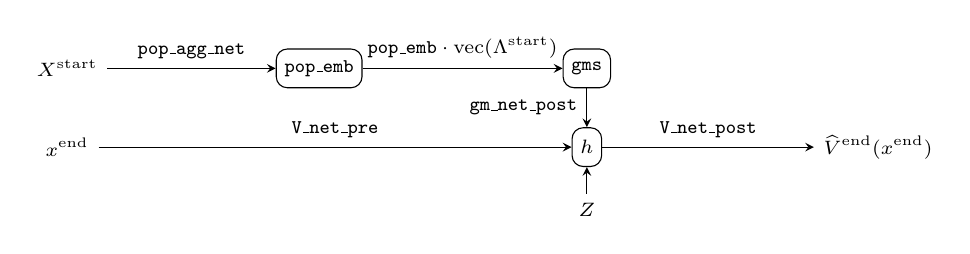
\begin{tikzpicture}[
    >=stealth,
    every node/.style={font=\scriptsize},
    blk/.style={draw, rounded corners, inner sep=3pt, minimum height=14pt,
                font=\scriptsize\ttfamily},
  ]
    % 输入（左列）
    \node (Xstart) at (0,  1.0)  {$X^{\mathrm{start}}$};
    \node (xend)   at (0,  0)    {$\xend$};
    \node (Z)      at (6.6, -0.8)  {$Z$};

    % 顶行
    \node[blk] (popemb) at (3.2, 1.0) {pop\_emb};
    \node[blk] (gms)    at (6.6, 1.0) {gms};

    % 中行
    \node[blk] (h)      at (6.6, 0)   {$h$};
    \node      (Vend)   at (10.3, 0)  {$\Vendhat(\xend)$};

    % 箭头
    \draw[->] (Xstart) -- node[above] {\texttt{pop\_agg\_net}} (popemb);
    \draw[->] (popemb) -- node[above] {$\texttt{pop\_emb}\cdot\mathrm{vec}(\Lstart)$} (gms);
    \draw[->] (xend)   -- node[above] {\texttt{V\_net\_pre}} (h);
    \draw[->] (gms)    -- node[left] {\texttt{gm\_net\_post}} (h);
    \draw[->] (Z)      -- (h);
    \draw[->] (h)      -- node[above] {\texttt{V\_net\_post}} (Vend);
  \end{tikzpicture}\par}

  \vspace*{-2.5em}
  四个子网络：
  \begin{enumerate}
    \item \texttt{pop\_agg\_net} $: (b, z) \to \R^{k}$ —— 逐格嵌入，对 $\Lstart$ 加权聚合，得到全局矩 $gms = \sum_{(b,z)} \Lambda(b, z) \cdot \texttt{pop\_agg\_net}(b, z) \in \R^k$。
    \item \texttt{V\_pre} $: (b, z) \to \R^m$ —— 为值函数头部提供的格级特征。
    \item \texttt{gm\_post} $: \R^k \to \R^m$ —— 将 $gms$ 投射到值函数头部的中间空间；逐格加到 \texttt{V\_pre} 上。
    \item \texttt{V\_post} $: \R^{m + N_Z} \to \R$ —— 最终头部；接收加总后的特征以及 $Z$ 的独热编码，输出 $\Vendhat$。
  \end{enumerate}
\end{frame}

\begin{frame}[fragile]{代码中的神经网络}
  \begin{lstlisting}
  struct VNet{A, P, G, V}
      pop_agg_net :: A    # (b, z) → gm_dim         为 GM 提供的逐格嵌入
      V_pre       :: P    # (b, z) → mid            为 V 头部提供的逐格特征
      gm_post     :: G    # gm_dim → mid            将 GM 投射到中间空间
      V_post      :: V    # mid + N_Z → 1           组合 + Z，读出 V_end
  end

  function (net::VNet)(Λ::AbstractMatrix, Z_idx::Int, p::KSParams)
      pop_emb = net.pop_agg_net(HH_FEAT)          # (gm_dim, N_CELLS)
      gm      = pop_emb * Float32.(vec(Λ))        # (gm_dim,)   人口加权平均
      h_pre   = net.V_pre(HH_FEAT)                # (mid, N_CELLS)
      h_gm    = net.gm_post(gm)                   # (mid,)
      h       = h_pre .+ h_gm                     # 广播 → (mid, N_CELLS)
      pred    = net.V_post(vcat(h, Z_ROWS[Z_idx])) # (1, N_CELLS)
      return reshape(pred, p.N_b, length(p.z_grid))
  end
  \end{lstlisting}
\end{frame}

\begin{frame}[fragile]{前瞻算子 $\CL V_\theta$}
  \begin{lstlisting}
  function lookahead(hh, vnet::VNet, Λ_start::AbstractMatrix, Z_idx::Int, p::KSParams)
      V_end_now = Float64.(vnet(Λ_start, Z_idx, p))
      env_now   = make_env(hh; ks_prices(integrate_K(hh, Λ_start), p.Z_vals[Z_idx], p)...)
      backward!(hh, V_end_now, env_now)                  # 确定储蓄策略
      Λ_end = forward!(hh, Λ_start)

      V_end_label = zeros(Float64, p.N_b, length(p.z_grid))
      for Z_next in 1:N_Z
          V_start_next = inner_solve_backward(hh, vnet, Λ_end, Z_next, p)
          V_end_label .+= p.Π_Z[Z_idx, Z_next] .* V_start_next
      end
      return (; V_end_label, Λ_end)
  end
  \end{lstlisting}
\end{frame}

\begin{frame}[fragile]{训练损失}
  将 \texttt{target} $\equiv \Vendhat_i$ 视为固定标签，对 \texttt{vnet} 进行自动微分。

  \begin{lstlisting}
  function build_targets(hh, vnet::VNet, batch, p::KSParams)
      targets = NamedTuple{(:Λ, :Z_idx, :target), Tuple{Matrix{Float64}, Int, Matrix{Float32}}}[]
      for (Λ_start, Z_idx) in batch
          out = lookahead(hh, vnet, Λ_start, Z_idx, p)
          push!(targets, (; Λ=copy(Λ_start), Z_idx, target=Float32.(out.V_end_label)))
      end
      return targets
  end

  function bellman_residual_loss(vnet::VNet, targets, p::KSParams)
      L = 0f0
      for (Λ, Z_idx, target) in targets
          pred  = vnet(Λ, Z_idx, p)
          scale = max(var(target), 1f-6)             # 按目标尺度归一化
          L    += sum((pred .- target).^2) / (length(pred) * scale)
      end
      return L / length(targets)
  end
  \end{lstlisting}
\end{frame}

\begin{frame}[fragile]{对 $\Lstart$ 采样}
  MCMC 风格：在给定\emph{当前} $V_\theta$ 的条件下进行模拟，预烧（burn in），然后子采样。

  \begin{lstlisting}
  function sim_one_step(hh, vnet::VNet, Λ::AbstractMatrix, Z_idx::Int, p::KSParams)
      V_end = Float64.(vnet(Λ, Z_idx, p))
      env   = make_env(hh; ks_prices(integrate_K(hh, Λ), p.Z_vals[Z_idx], p)...)
      backward!(hh, V_end, env)
      return forward!(hh, Λ)
  end

  function sample_ergodic(hh, vnet::VNet, p::KSParams; T=200, burn=100, every=2, rng=MersenneTwister(8421))
      Λ     = copy(Λ_ss)
      Z_idx = 1
      batch = Tuple{Matrix{Float64}, Int}[]
      for t in 1:T
          Λ     = sim_one_step(hh, vnet, Λ, Z_idx, p)
          Z_idx = sample_Z(Z_idx, p.Π_Z, rng)
          if t > burn && (t - burn) % every == 0
              push!(batch, (copy(Λ), Z_idx))
          end
      end
      return batch
  end
  \end{lstlisting}
\end{frame}

\begin{frame}[fragile]{训练循环}
  \begin{lstlisting}
  function train!(vnet::VNet, hh, p::KSParams; epochs=50, lr=1e-3, T=200, burn=100, every=4)
      opt  = Flux.setup(Adam(lr), vnet)
      hist = Float64[]
      rng  = MersenneTwister(1729)
      for epoch in 1:epochs
          batch   = sample_ergodic(hh, vnet, p; T, burn, every, rng=MersenneTwister(rand(rng, UInt32)))
          targets = build_targets(hh, vnet, batch, p)
          loss, grads = withgradient(vnet) do net
              bellman_residual_loss(net, targets, p)
          end
          Flux.update!(opt, vnet, grads[1])
          push!(hist, Float64(loss))
      end
      return hist
  end
  \end{lstlisting}
\end{frame}

\begin{frame}[fragile]{初始化与预训练}
  在扰动后的 $\Lambda_{\mathrm{ss}}$ 和所有 $Z$ 上，对 $V_{\mathrm{ss}}$ 进行预训练。
  \begin{lstlisting}
  function perturb_Λ(Λ::AbstractMatrix, σ, rng)
      Λp = Λ .* (1 .+ σ .* randn(rng, size(Λ)))
      Λp = max.(Λp, 0)
      return Λp ./ sum(Λp)
  end

  function pretrain_to_ss!(vnet::VNet, V_ss_target, p::KSParams; epochs=300, lr=5e-3, n_Λ=6, σ=0.10, seed=4747)
      opt    = Flux.setup(Adam(lr), vnet)
      target = Float32.(V_ss_target)
      rng    = MersenneTwister(seed)
      hist   = Float64[]
      for epoch in 1:epochs
          Λ_cloud = [perturb_Λ(Λ_ss, σ, rng) for _ in 1:n_Λ]
          loss, grads = withgradient(vnet) do net
              L = 0f0
              for Λ in Λ_cloud, Z_idx in 1:N_Z
                  pred = net(Λ, Z_idx, p)
                  L += sum((pred .- target).^2)
              end
              L / (n_Λ * N_Z * length(target))
          end
          Flux.update!(opt, vnet, grads[1])
          push!(hist, Float64(loss))
      end
      return hist
  end
  \end{lstlisting}
\end{frame}

% =============================================================
\section[推广]{推广}
% =============================================================

\begin{frame}{推广：模型}
  \begin{itemize}
    \item 对任何能够实现 $\Phi$ 的模型，这一通用方法都是良定义的。
    \item 如果你无法实现 $\Phi$，那么问题并不在于总量不确定性。
    \item 我提供了 \texttt{HouseholdStages.jl}，用于构建高性能的家庭模块。
    \item 可以处理：空间、多部门、世代交叠（OLG）、搜寻—匹配、新凯恩斯、带摩擦的耐用资产（如住房）、理性疏忽、Epstein--Zin 偏好
  \end{itemize}
\end{frame}

\begin{frame}{推广：分割市场}
  分割市场模型，例如包含多个区位或多个部门的模型，带来了额外的挑战。

  我提出：
  \begin{itemize}
    \item \textbf{分割广义矩}，将 Han--Yang--E (2025) 推广为以模型一致的方式同时压缩分段（如区位）数据与总量数据。
    \item \textbf{轻量网络头部}方法，将含 $n$ 个分段、$m$ 个家庭状态的分割市场模型的训练，从 $O(nm)$ 加速到实质上的 $O(n+m)$
  \end{itemize}
\end{frame}

\begin{frame}{推广：方法}
  原则上，nVFI 算法并不依赖于以下这些实现细节：
  \begin{itemize}
    \item $\CV_\theta$ 的参数化：我使用神经网络，但该方法只需要某种可训练的函数近似器。
    \item 值函数的表示：我使用在离散化特异性状态上的矩阵，但你也可以使用样条、Chebyshev 多项式，甚至另一个神经网络。
    \item 人口的表示：我使用在离散化特异性状态上的矩阵，但你也可以使用矩、有限主体等。
    \item 期内求解器：我主要使用基于网格的方法，但你也可以使用 EGM、Reiter 等。
  \end{itemize}
  只要你能实现\textbf{期内求解器} $\Phi$，该算法就是良定义的。
\end{frame}

\begin{frame}{与 HouseholdStages.jl 的关系}
  本方法与我在 Household Stages 上的工作之间存在如下深层联系：
  \begin{itemize}
    \item 离散时间的异质性主体（HA）模型具有基于\textbf{函数复合}的\textbf{复合结构}
    \item 相比之下，连续时间的 HA 模型具有基于\textbf{可加复合}的复合结构。
  \end{itemize}
  关于 Household Stages 的论文与软件包探讨了这一点对\textbf{期内求解器} $\Phi$ 的意涵

  受此启发，nVFI 用 $\CV$ 推广了贝尔曼方程，并将其用于全局求解。
\end{frame}

\end{document}
